\documentclass[12pt,letterpaper]{article}
\usepackage[utf8]{inputenc}
\usepackage{pgfplots} %Paquete para crear gráficas de funciones matemáticas basadas en PGF/TikZ
\usepackage[hidelinks]{hyperref}
\author{Curso de \LaTeX}
\title{Graficar funciones con pgfplots}
\begin{document}
\maketitle
PGF/TikZ también tiene un motor de matemáticas que le permite graficar funciones. El paquete de  \texttt{pgfplots} nos facilita este trabajo, incorporando un conjunto de entornos y macroinstrucciones basadas en PGF/TikZ, que están especialmente diseñadas para la graficación de funciones matemáticas. Por ejemplo, para graficar la función $y = x^2$ crearíamos un entorno \texttt{tikzpicture} como el siguiente:

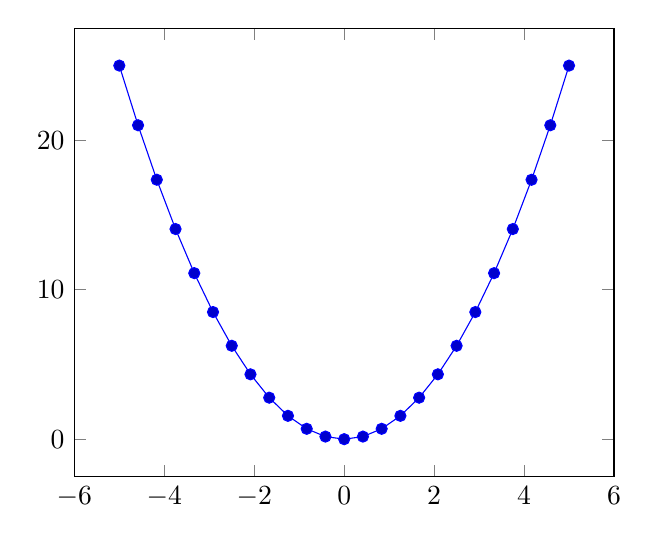
\begin{tikzpicture}
	\begin{axis}
		\addplot{x^2};
	\end{axis}
\end{tikzpicture}

El entorno \texttt{axis} nos permite dibujar un plano cartesiano para visualizar las coordenadas $x$ y $y$ del gráfico, mientras que el comando \texttt{\textbackslash addplot} nos permite añadir la función matemática a graficar.

Podemos añadir algunas opciones de TikZ al comando \texttt{\textbackslash addplot}:

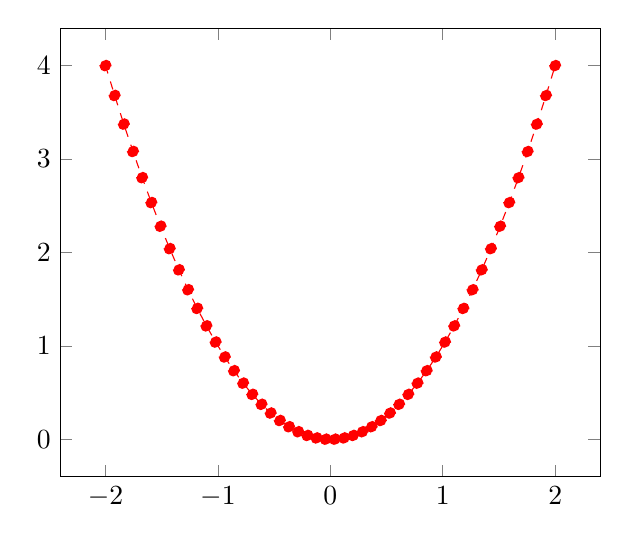
\begin{tikzpicture}
	\begin{axis}
		\addplot[color=red, dashed, mark=*, samples=50,domain=-2:2]{x^2};
	\end{axis}
\end{tikzpicture}

Como vemos, la opción \texttt{samples} permite definir el número de muestras de la variable $x$ para la función, mientras que \texttt{domain} define su dominio (rango de valores para $x$).

También podemos modificar la apariencia de los ejes del gráfico cambiando sus rangos y utilizando sólo dos líneas: 

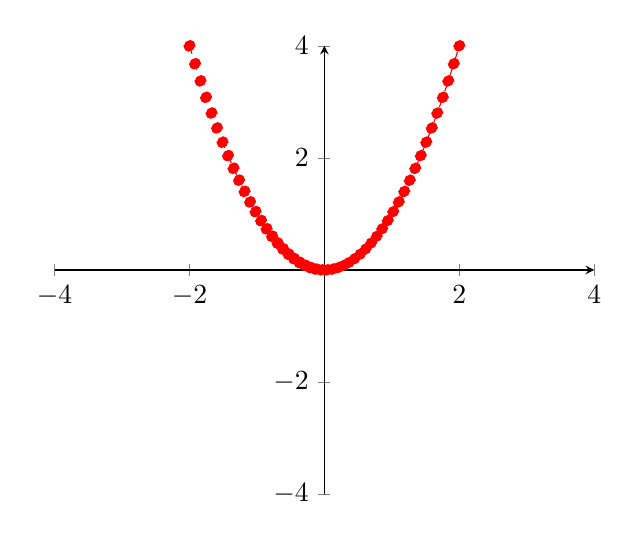
\begin{tikzpicture}
	\begin{axis}[xmin=-4, xmax=4, ymin=-4, ymax=4, axis lines=middle]
		\addplot[color=red, dashed, mark=*, samples=50,domain=-2:2]{x^2};
	\end{axis}
\end{tikzpicture}

Como vemos, las opciones \texttt{xmin}, \texttt{xmax}, \texttt{ymin} y \texttt{ymax} definen los rangos de las coordenadas de los ejes, mientras que \texttt{axis lines} define la forma en la que se mostrarán los ejes del gráfico. Ésta opción acepta los valores \texttt{left}, \texttt{right} y \texttt{middle}.

Hay muchas funciones matemáticas disponibles para incorporar a nuestras gráficas, aquí hay una selección: \texttt{factorial(x), sqrt(x), pow(x,y), exp(x), ln(x), log10(x), log2(x), abs(x), mod(x,y), round(x), floor(x), ceil(x), sin(x), cos(x), tan(x)}. 

Un ejemplo con tres funciones defiendo el mismo dominio para todas:

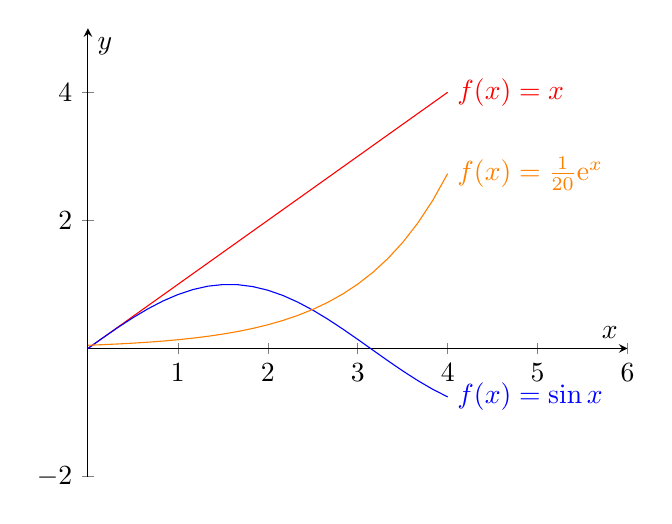
\begin{tikzpicture}[domain=0:4]
	\begin{axis}[xmin=0, xmax=6, ymin=-2, ymax=5, axis lines=middle, xlabel=$x$, ylabel=$y$]
		\addplot[color=red]{x} node[right] {$f(x) =x$}; 
		\addplot[color=blue]{sin(deg(x))} node[right] {$f(x) = \sin x$}; 
		\addplot[color=orange]{0.05*exp(x)} node[right] {$f(x) = \frac{1}{20} \mathrm e^x$};
	\end{axis}
\end{tikzpicture}

También podemos crear polígonos a partir de funciones, cerrando las curvas con el comando \texttt{\textbackslash closedcycle}. Por ejemplo, podemos crear un polígono utilizando la función $f(x) = 4-x^2$:

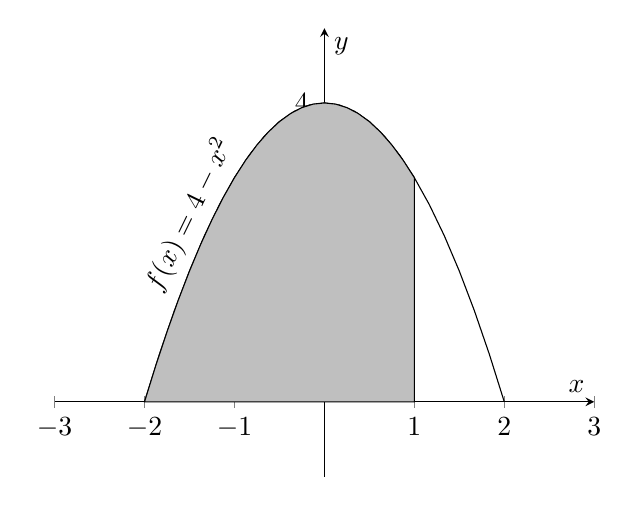
\begin{tikzpicture}
	\begin{axis}[xmin=-3, xmax=3, ymin=-1, ymax=5, axis lines=middle, xlabel=$x$, ylabel=$y$]
		\addplot[domain=-2:2]{4-x^2}; 
		\addplot[domain=-2:1,fill=lightgray]{4-x^2}\closedcycle; 
		\node [rotate=64] at (axis cs: -1.5,  2.5) {$f(x) = 4-x^2$};
	\end{axis}
\end{tikzpicture}

Y finalmente, es posible graficar funciones con tres variables con el comando \texttt{\textbackslash addplot3} generando un gráfico tridimensional, por ejemplo para la función $z = 1-x^2-y^2$:

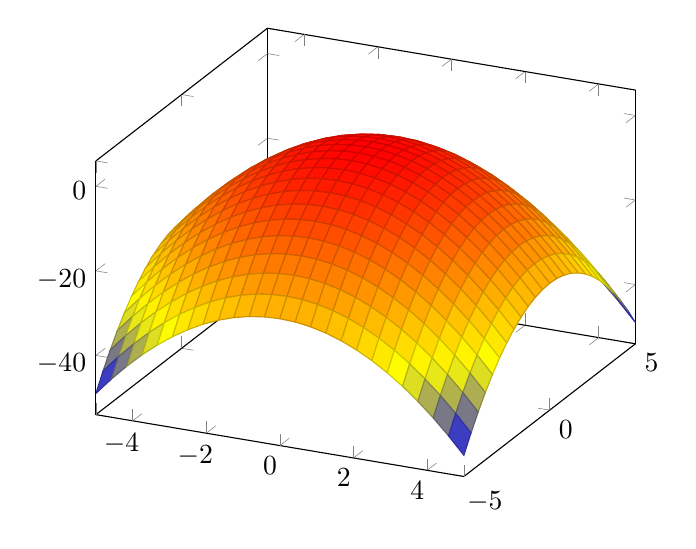
\begin{tikzpicture}
	\begin{axis}
		\addplot3[surf]{1-x^2-y^2}; 
	\end{axis}
\end{tikzpicture}

La opción \texttt{surf} indica que el gráfico tendrá un color de relleno para su superficie, con un gradiente de color que recuerda a un mapa topográfico.

Para conocer todas las capacidades del paquete pgfplots, puedes revisar su documentación completa en el siguiente enlace: \url{https://mirror.mwt.me/ctan/graphics/pgf/contrib/pgfplots/doc/pgfplots.pdf}

Para conocer más ejemplos y comandos avanzados del paquete TikZ, puedes consultar su documentación oficial en: \url{https://texample.net/media/pgf/builds/pgfmanualCVS2012-11-04.pdf }.

Además, existe un amplio catálogo de gráficos creados con este paquete, disponible para utilizarlo libremente en el sitio: \url{https://texample.net/tikz/}
\end{document}